\chapter{Empirische Verarbeitung}
\label{chap:Empirie}

\section{Methodik}
\label{sec:Methodik}

Im folgenden Kapitel werde ich die der Studie zugrunde gelegten Daten präsentieren, ihre Auswahl begründen, und ihre Beschaffung und Bereinigung beschreiben. Im Anschluss werde ich die Social Web Beiträge nach den in \ref{sec:jhsforschung} erarbeiteten Kriterien in die Funktionsgruppen des Modells von Jan-Hinrik Schmidt einordnen, so dies denn möglich ist.

\subsection{Daten}
\label{sec:Daten}

\subsubsection{Datenauswahl}
\label{sec:Datenauswahl}

Der untersuchte Datensatz umfasst die Social Web Beiträge, die von der Universität Bielefeld selbst im Zeitraum vom 01. Juli 2018 bis einschließlich 31. Juli 2018 jeweils auf den Plattformen Instagram, YouTube, Twitter, Facebook, Universitäts-Blog veröffentlicht worden sind. Der einmonatige Zeitraum wurde gewählt, um eine noch analysierbare, jedoch aussagekräftige Beitrags-Menge zu erhalten. Der spezifische Zeitraum liegt im Übergang von Vorlesungszeit zu vorlesungsfreier Zeit, damit ein eventueller Unterschied zwischen den beiden Perioden dargestellt werden kann.

\subsubsection{Beschaffung}
\label{sec:Datenbeschaffung}

Die Facebook-Beiträge wurden mit Hilfe der Facebook Graph API\footnote{Facebook Graph API - \url{https://developers.facebook.com/tools/explorer} - Eine Programmierschnittstelle zur automatisierten Datenbeschaffung} im in der automatisierten Datenverarbeitung üblichen JSON-Format heruntergeladen, um die Text-Beiträge von der grafischen Oberfläche unabhängig darstellen zu können. Für die Twitter-Beiträge wurde die Twitter Search API\footnote{Twitter Search API - \url{https://twitter.com/search-advanced}} genutzt, um ebenselben Effekt zu erzielen. Aufgrund der weniger umfangreichen Beitragszahl, wurde die Liste der YouTube-Beiträge händisch erstellt. Selbes gilt für die Instagram-Beiträge. Die Blog-Beiträge des Universitäts-Blogs wurden ebenfalls händisch heruntergeladen, da das genutzte Blogsystem keine Programmierschnittstelle zur Verfügung stellt.

Zusätzlich zu den Text-Varianten, wurden grafische Darstellungen aller Beiträge erstellt und im Anhang archiviert.

\subsubsection{Bereinigung}
\label{sec:Datenbereinigung}

Die Facebook-Beiträge wurden so bereinigt, dass nur noch Inhalt, Reaktionszahlen (Like, etc.), Kommentarzahlen und eine Info vorhanden sind, ob dem Text-Beitrag ein weiteres Medium hinzugefügt wurde; und wenn ja, welches (Bild, Video, Link, Veranstaltungseinladung). Bei den Twitter-Beiträgen wurden neben dem Inhalt die Interaktionsdaten zu Kommentaren, Retweets und Likes aufgenommen. Für die Instagram-Beiträge wurden die Beschreibung des Bildes/Videos, die Zahlen der Likes und die Zahlen der Kommentare aufgenommen. Die YouTube-Videos wurden mit Videobeschreibung, View- und Like-, sowie Kommentarzahlen notiert. Da beim Universitäts-Blog die Kommentarfunktion nicht aktiviert ist, wurden hier nur die Beiträge in den Datensatz aufgenommen.

\subsubsection{Datensatz}
\label{sec:Datensatz}

Der gesamte Datensatz umfasst 105 Beiträge, von denen in aufsteigender Reihenfolge sieben auf Twitter, elf auf YouTube, 22 auf Instagram, 29 im Universitäts-Blog und 36 auf Facebook veröffentlicht wurden.

\begin{figure}[h]
    \centering
    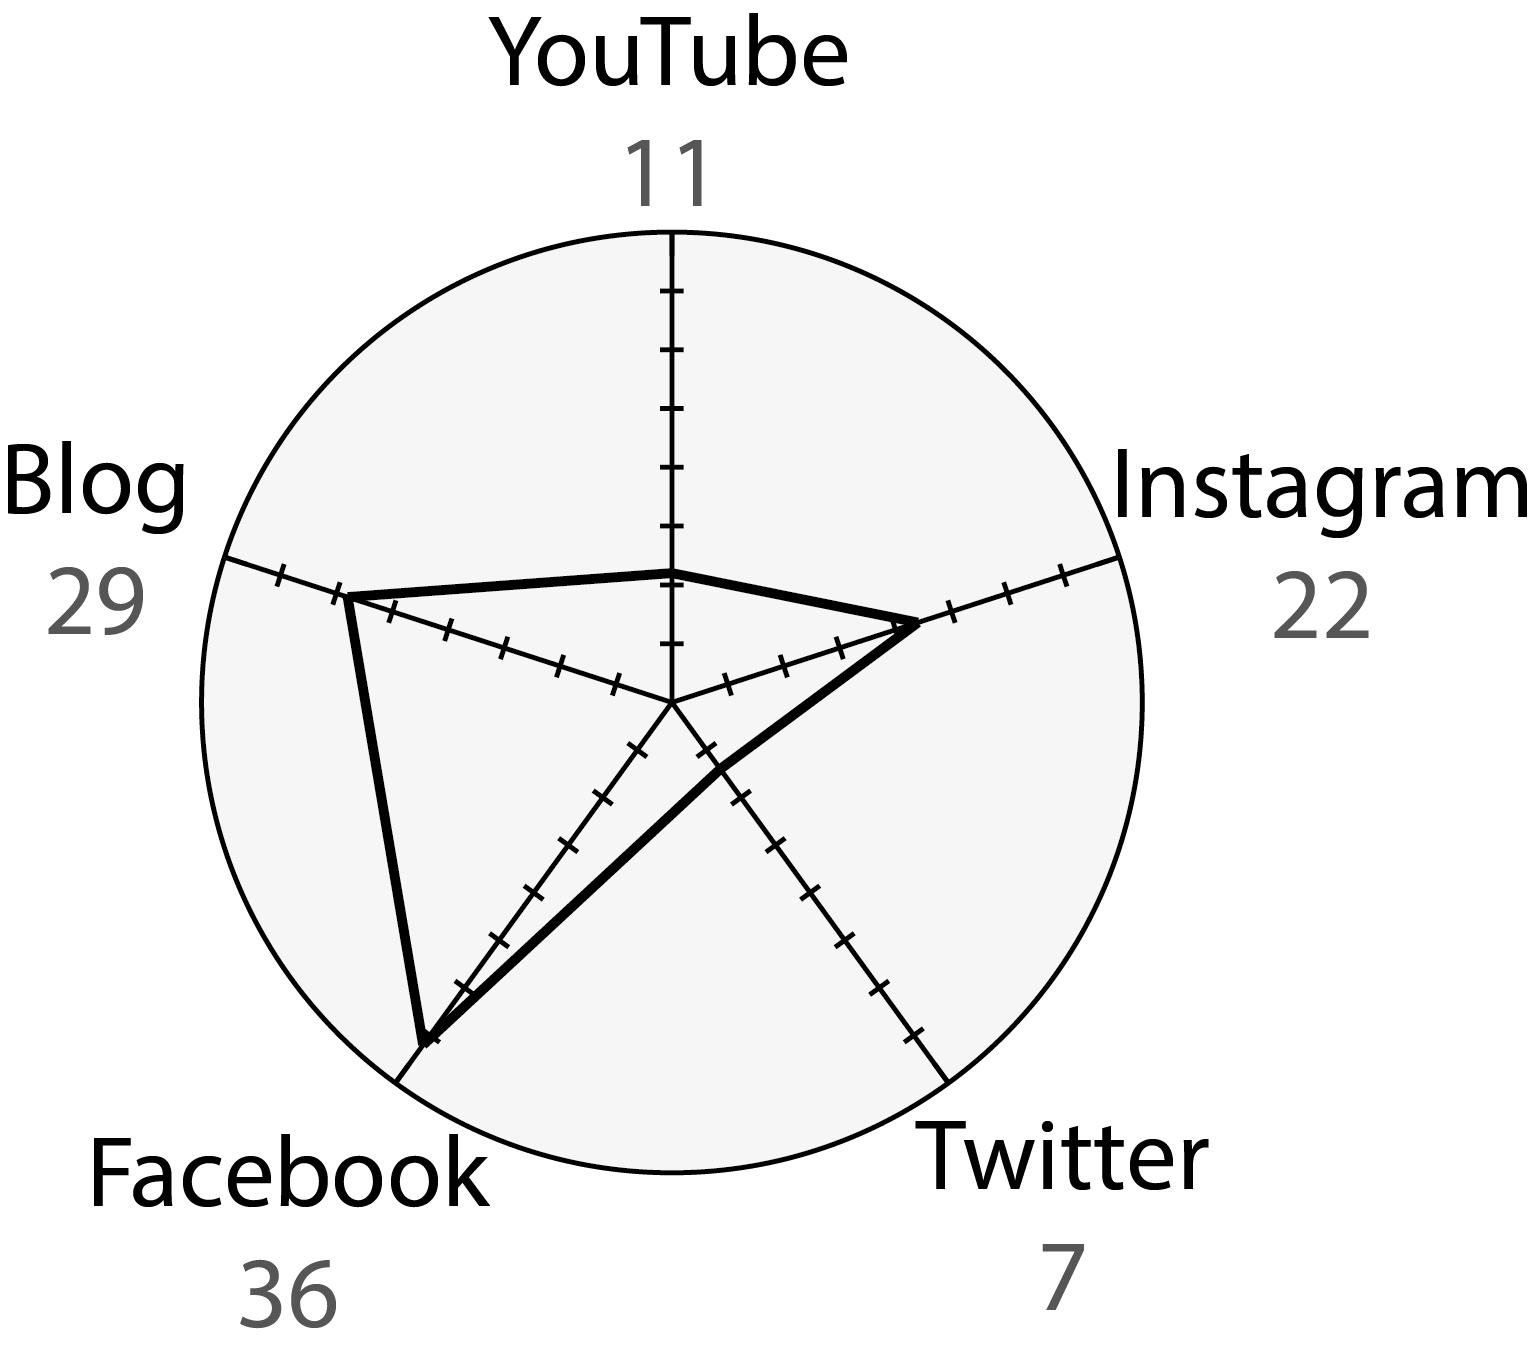
\includegraphics[width=.6\textwidth]{img/posts/posts_gesamt.png}
    \caption{Social Web Beiträge der Universität Bielefeld im Juli 2018. Der Radar-Graph zeigt einen Überhang an Facebook- und Blog-Beiträgen und ein Minimum an Twitter-Beiträgen.}
    \label{fig:socialmediaposts}
\end{figure}  

Dabei sind die Blog-Beiträge, mit durchschnittlich knapp 400 Worten, die längsten Beiträge, wie dem Boxplot in Abbildung \ref{fig:wortlaengebl} zu entnehmen ist.

\begin{figure}[h]
    \centering
    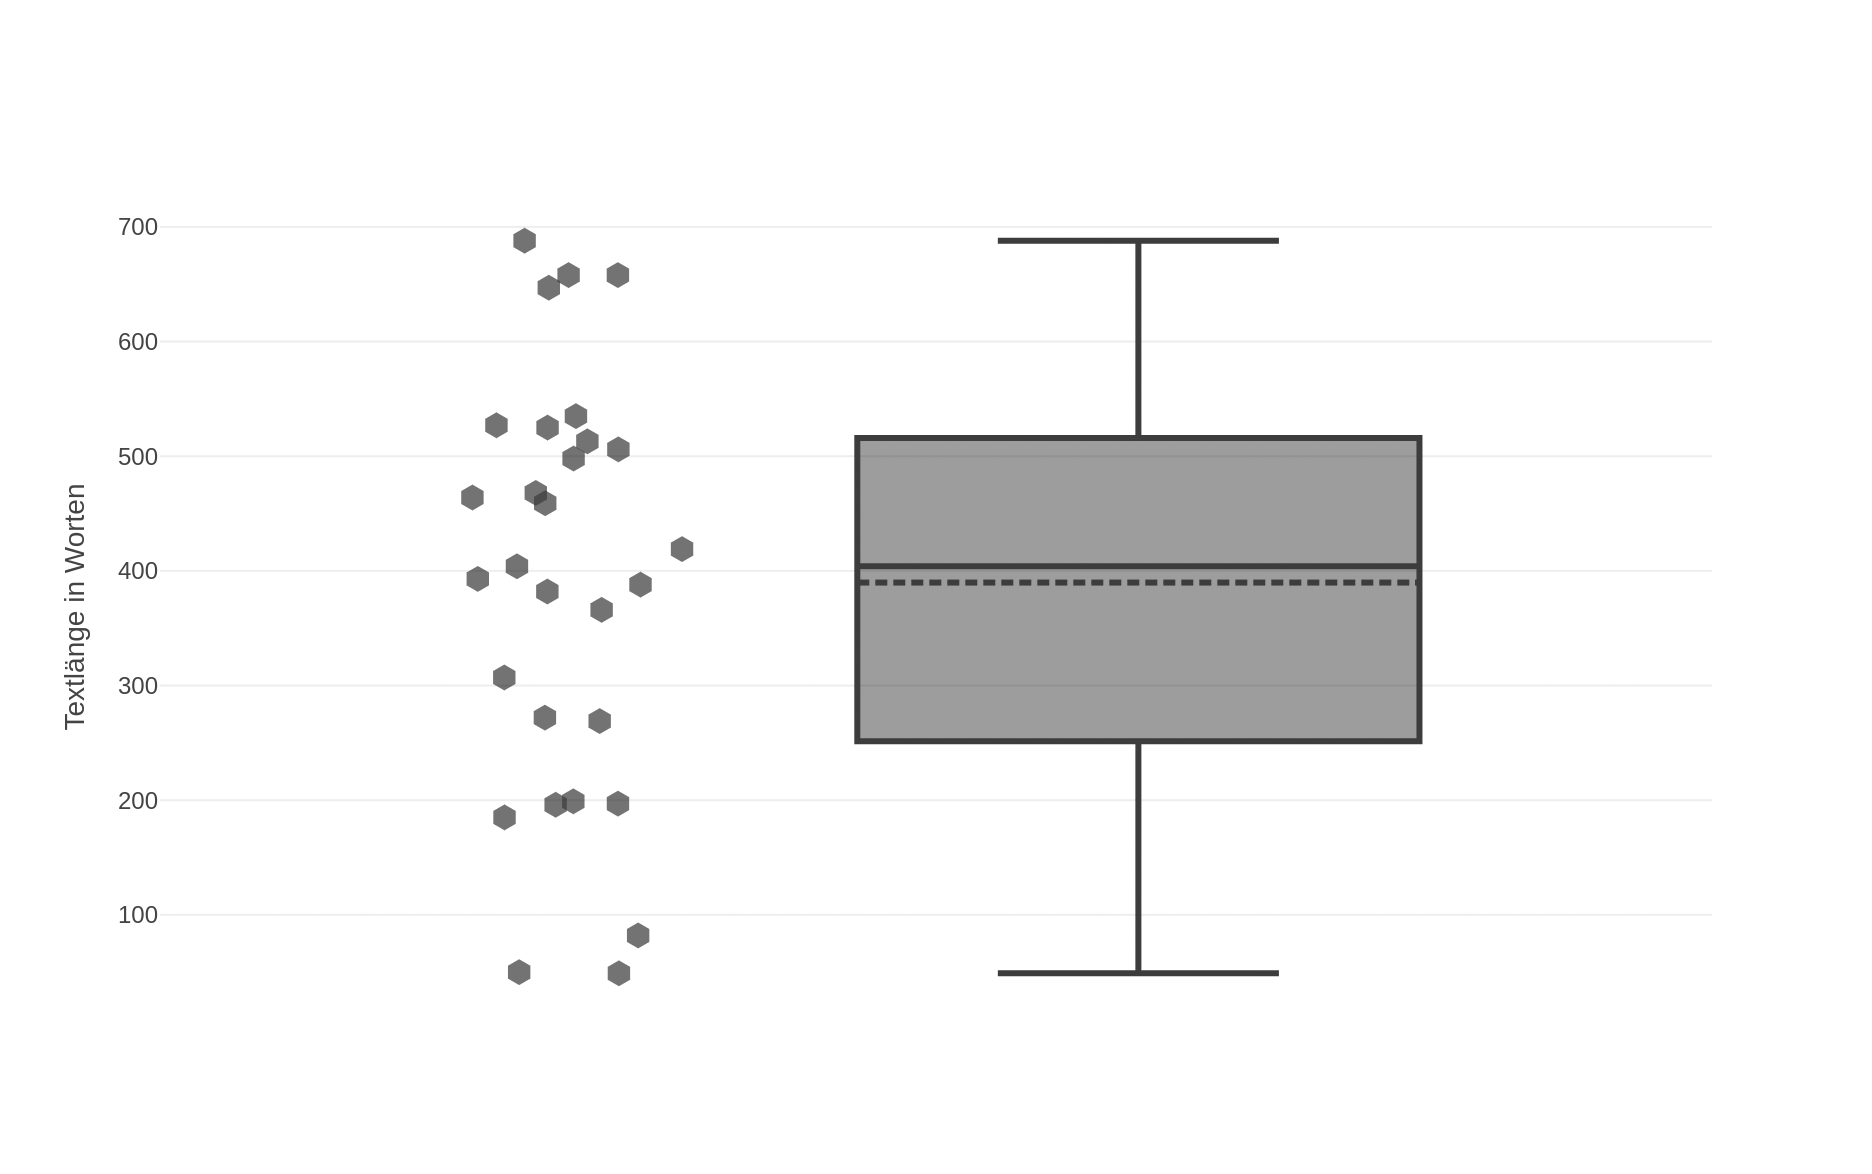
\includegraphics[width=\textwidth]{img/plots/bl.png}
    \caption{Textlänge der Blog-Beiträge in einem Boxplot-Diagramm. Die gestrichelte Linie zeigt den Durchschnitt, die darüber liegende Linie den Median an. Das Minimum liegt bei 49, das Maximum bei 688 Worten.}
    \label{fig:wortlaengebl}
\end{figure}

Die Beitragslängen im Blog reichen von 49 bis zu 688 Worten, erreichen bei etwa 390 Worten den Durchschnitt und bei knapp 404 Worten den Median. Daraus ergibt sich eine Standardabweichung von 182.28.

\begin{figure}[h]
    \centering
    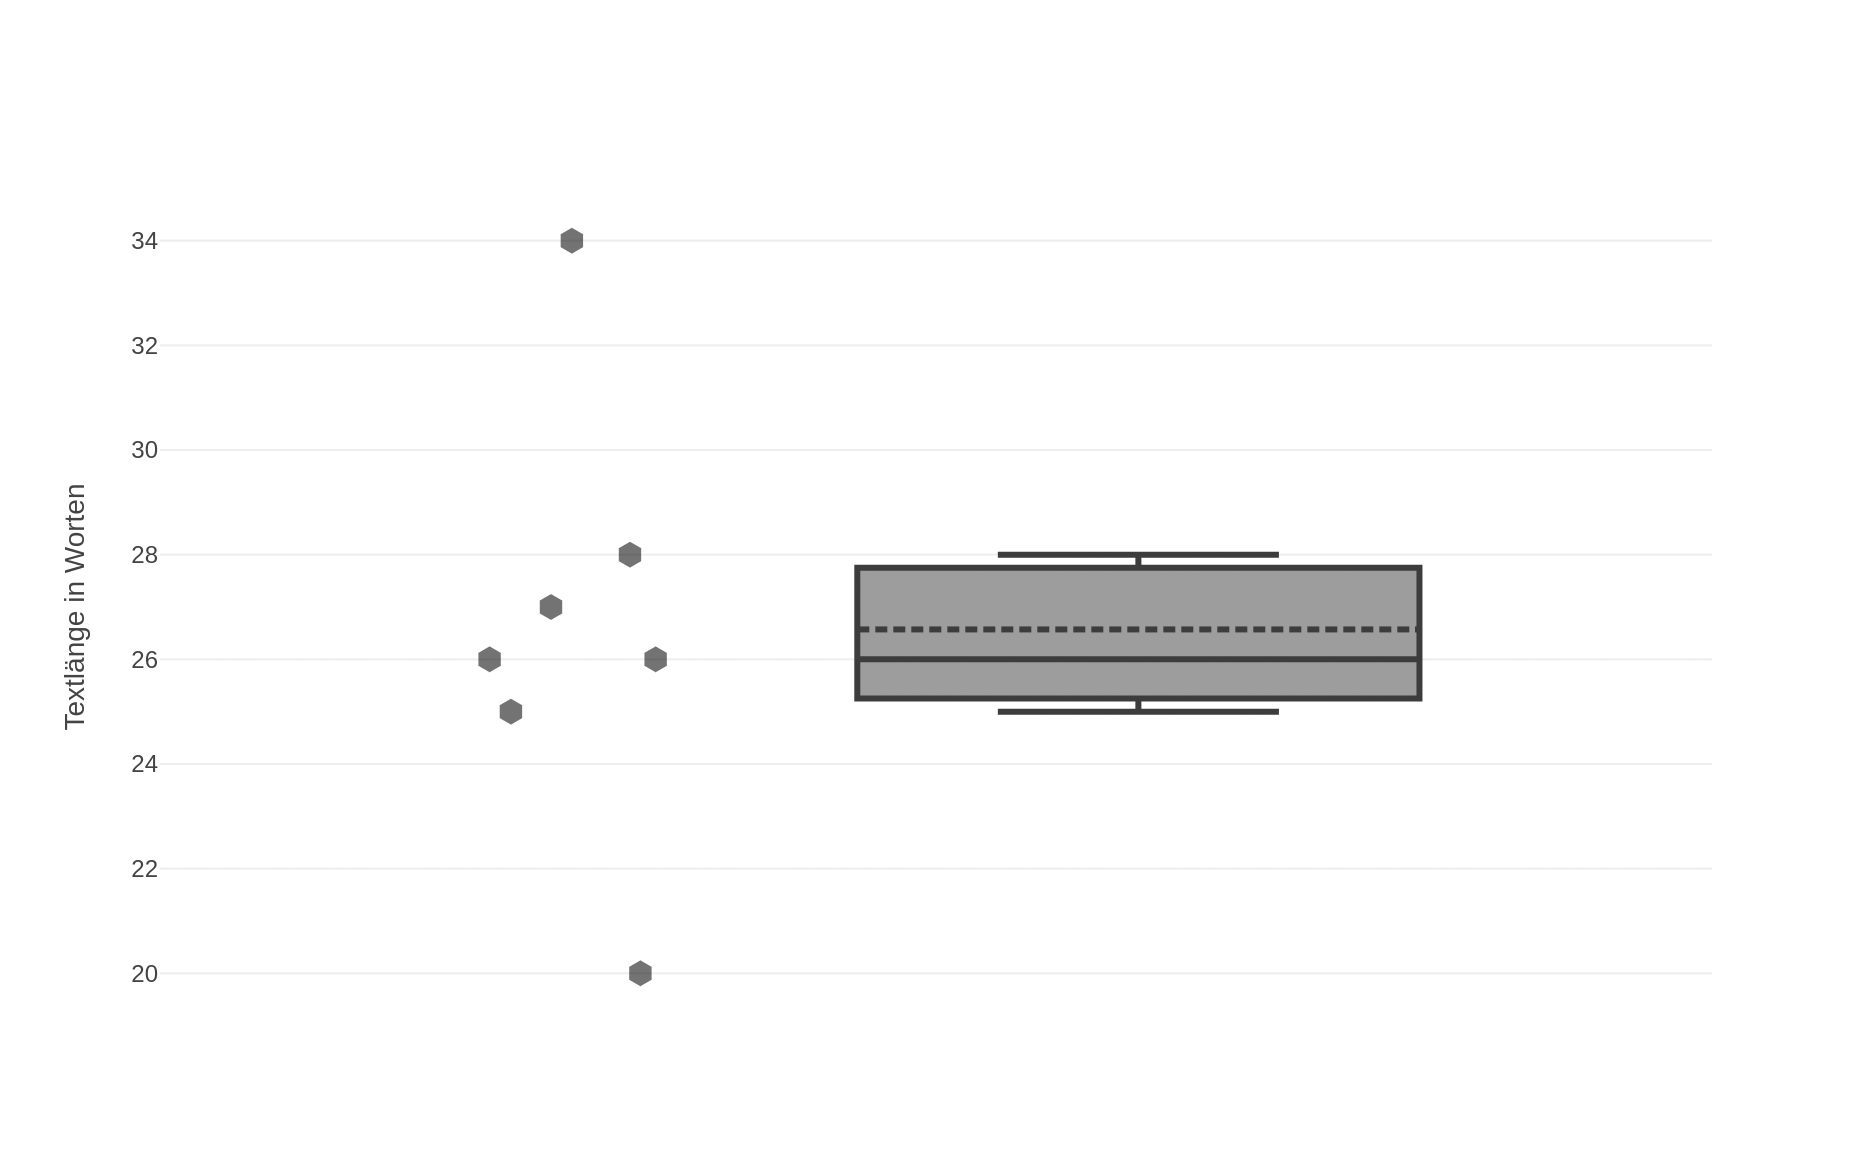
\includegraphics[width=\textwidth]{img/plots/tw.png}
    \caption{Textlänge der Twitter-Beiträge in einem Boxplot-Diagramm, welche den technischen Einschränkungen der Plattform nach erwartungsgemäß eine niedrige Standardabweichung aufzeigen.}
    \label{fig:wortlaengetw}
\end{figure}

\begin{figure}[h]
    \centering
    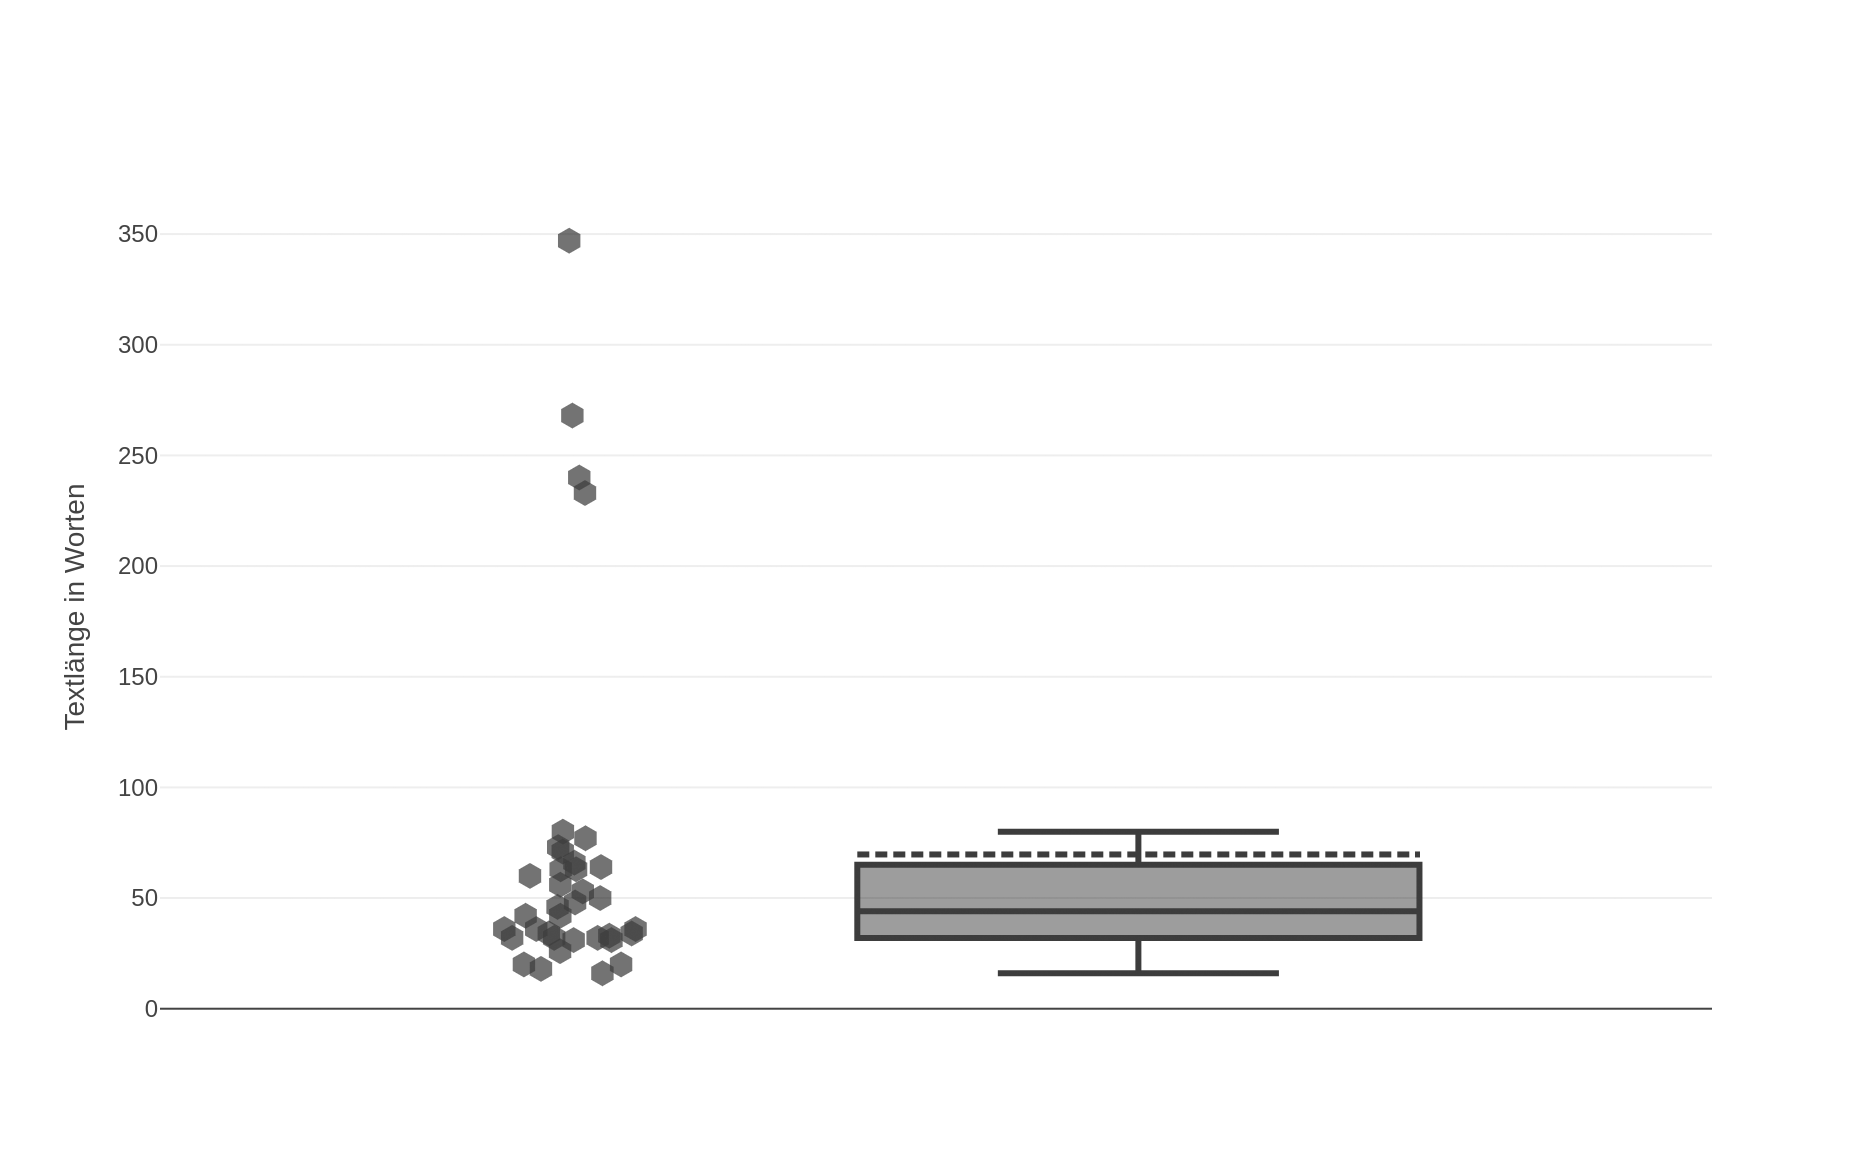
\includegraphics[width=\textwidth]{img/plots/fb.png}
    \caption{Textlänge der Facebook-Beiträge. In der Box ist der Median durch die durchgezogene Linie angezeigt. Die gestrichelte Linie zeigt den Durchschnitt, der durch die Ausreißer am oberen Rand des Spektrums über die Box hinausgeht. Hier reicht die Textlänge von 16 Worten bis hin zu 347 Worten}
    \label{fig:wortlaengefb}
\end{figure}

In den Abbildungen \ref{fig:wortlaengetw} \& \ref{fig:wortlaengefb} sind Boxplots der Textlängen von respektive Twitter- und Facebook-Beiträgen dargestellt.

Die Twitter-Beiträge bewegen sich zwischen 20 und 34 Worten. Der Durchschnitt liegt bei knapp 27 und der Median bei knapp 26 Worten. Die Standardabweichung ist mit knapp vier Worten sehr viel kleiner als die der Blog- und Facebook-Beiträge. Dies ist sehr deutlich in Abbildung \ref{fig:wortlaengetw} zu erkennen.

Wie in Abbildung \ref{fig:wortlaengefb} zu sehen, reichen die Beiträge von Facebook von 16 bis zu 347 Worten. Im Durchschnitt hat ein Facebook-Beitrag knapp 70 Worte. Der Median liegt bei 44 und die Standardabweichung mit 76 Worten zwischen denen der Twitter- und Blog-Beiträge. Alle Ausreißer der Facebook-Beiträge sind dem Beitrags-Format \textit{Meine Uni - Mein Thema} zuzuordnen.

Da es sich bei YouTube und Instagram im Kern nicht um textbasierte Plattformen handelt, wurden die oben aufgezeigten Statistiken für diese Plattformen nicht ausgeführt.


\subsection{Einteilung der Social Web Posts der Universität Bielefeld in die Management-Leistungen nach Jan-Hinrik Schmidt}
\label{sec:jhseinteilung}

Die auf Text basierten Social Web Beiträge der Universität Bielefeld sollen in diesem Abschnitt in die von Jan-Hinrik Schmidt eingeführten Leistungen Identitätsmanagement (\texttt{ID}), Beziehungsmanagement (\texttt{BEZ}) und Informationsmanagement (\texttt{INFO}) eingeteilt werden. In den erstellten Tabellen sind den Beiträgen jeweils UIDs (Unique Identifiers) zugeordnet worden. Diese setzen sich nach dem Schema \texttt{SWP\_D\_C} zusammen. \texttt{SWP} ist das Kürzel der Social Web Plattform; \texttt{FB} für Facebook, \texttt{BL} für den Universitäts-Blog und \texttt{TW} für Twitter. \texttt{D} ist die zweistellige Darstellung des Tages innerhalb des Monats Juli 2018. \texttt{C} ist ein sogenannter Counter, also eine Zählvariable; für den Fall, dass an einem Tag mehrere Beiträge auf ein und derselben Plattform veröffentlicht wurden.

\texttt{TW\_16\_03} wäre demnach der dritte Beitrag, der am 16. Juli 2018 auf der Twitter-Seite der Universität Bielefeld veröffentlicht wurde.

In den Spalten \texttt{ID}, \texttt{BEZ} und \texttt{INFO} wird jeweils ein \texttt{X} eingetragen, wenn der Beitrag der jeweiligen Management-Leistung zugeordnet werden kann. Ist dies nicht der Fall, wird die Tabellen-Zelle leer gelassen.

\subsubsection{Facebook}

In der folgenden Tabelle \ref{tab:kategoriefb} sind in den Spalten die UIDs der Facebook-Beiträge der Universität Bielefeld aus dem Juli 2018 eingetragen, die sich wie oben in \ref{sec:jhseinteilung} beschrieben zusammensetzen. In den drei Datenzeilen ist eingetragen, ob der entsprechende Beitrag der angegebenen Management-Leistung zugeordnet werden kann. Wie folgend auch in \ref{fig:kategoriefb} zu sehen, ließen sich 20.9 \% der Beiträge zum Identitätsmanagement, 18.6 \% dem Beziehungsmanagement, und 60.5 \% dem Informationsmanagement zuteilen. Zu beachten ist, dass sowohl Einfach- als auch Mehrfachkategorisierungen möglich waren. Wie im rechten Teil der Abbildung \ref{fig:kategoriefb} zu sehen, konnten 16.7 \% aller Beiträge keiner der drei Management-Leistungen zugeordnet werden. 47.2 \% der Beiträge waren eindeutig zuordenbar; 36.1 \% konnten mehreren Kategorien zugeordnet werden.

\begin{table}[H]
    \caption{Facebook Beiträge der Universität Bielefeld im Juli 2018 und ihre Zuordnung zu den Management-Leistungen nach Schmidt.}
\resizebox{\textwidth}{!}{%
\begin{tabular}{*{36}{c|}c}
& \rotatebox{270}{FB\_02\_01} & \rotatebox{270}{FB\_02\_02} & \rotatebox{270}{FB\_03\_01 } & \rotatebox{270}{FB\_04\_01} & \rotatebox{270}{FB\_04\_02} & \rotatebox{270}{FB\_05\_01} & \rotatebox{270}{FB\_05\_02} & \rotatebox{270}{FB\_05\_03} & \rotatebox{270}{FB\_06\_01} & \rotatebox{270}{FB\_06\_02} & \rotatebox{270}{FB\_09\_01} & \rotatebox{270}{FB\_10\_01} & \rotatebox{270}{FB\_11\_01} & \rotatebox{270}{FB\_12\_01} & \rotatebox{270}{FB\_12\_02} & \rotatebox{270}{FB\_13\_01} & \rotatebox{270}{FB\_13\_02} & \rotatebox{270}{FB\_16\_01} & \rotatebox{270}{FB\_17\_01} & \rotatebox{270}{FB\_18\_01} & \rotatebox{270}{FB\_18\_02} & \rotatebox{270}{FB\_19\_01} & \rotatebox{270}{FB\_20\_01} & \rotatebox{270}{FB\_20\_02} & \rotatebox{270}{FB\_23\_01} & \rotatebox{270}{FB\_24\_01} & \rotatebox{270}{FB\_24\_02} & \rotatebox{270}{FB\_25\_01} & \rotatebox{270}{FB\_26\_01} & \rotatebox{270}{FB\_26\_02} & \rotatebox{270}{FB\_27\_01} & \rotatebox{270}{FB\_27\_02} & \rotatebox{270}{FB\_27\_03} & \rotatebox{270}{FB\_30\_01} & \rotatebox{270}{FB\_30\_02} & \rotatebox{270}{FB\_31\_01} \\
\hline
 ID & &  &  &  &  & X & X &  &  & X &  & X & X &  &  &  & X &  &  &  &  &  &  &  &  &  &  &  & X &  &  & X &  &  & X &  \\
 \hline
 BEZ & & X & X & X &  & X &  & X & X &  &  & X &  &  &  &  &  &  &  &  &  &  & X &  &  &  &  &  &  &  &  &  &  &  &  &  \\
 \hline
 INFO & & X & X & X & X &  & X & X & X & X &  & X &  & X & X & X & X &  & X &  &  & X &  & X &  & X & X & X & X & X & X & X & X &  & X & X
\end{tabular}%
}
\label{tab:kategoriefb}
\end{table}

\begin{figure}[H]
    \centering
    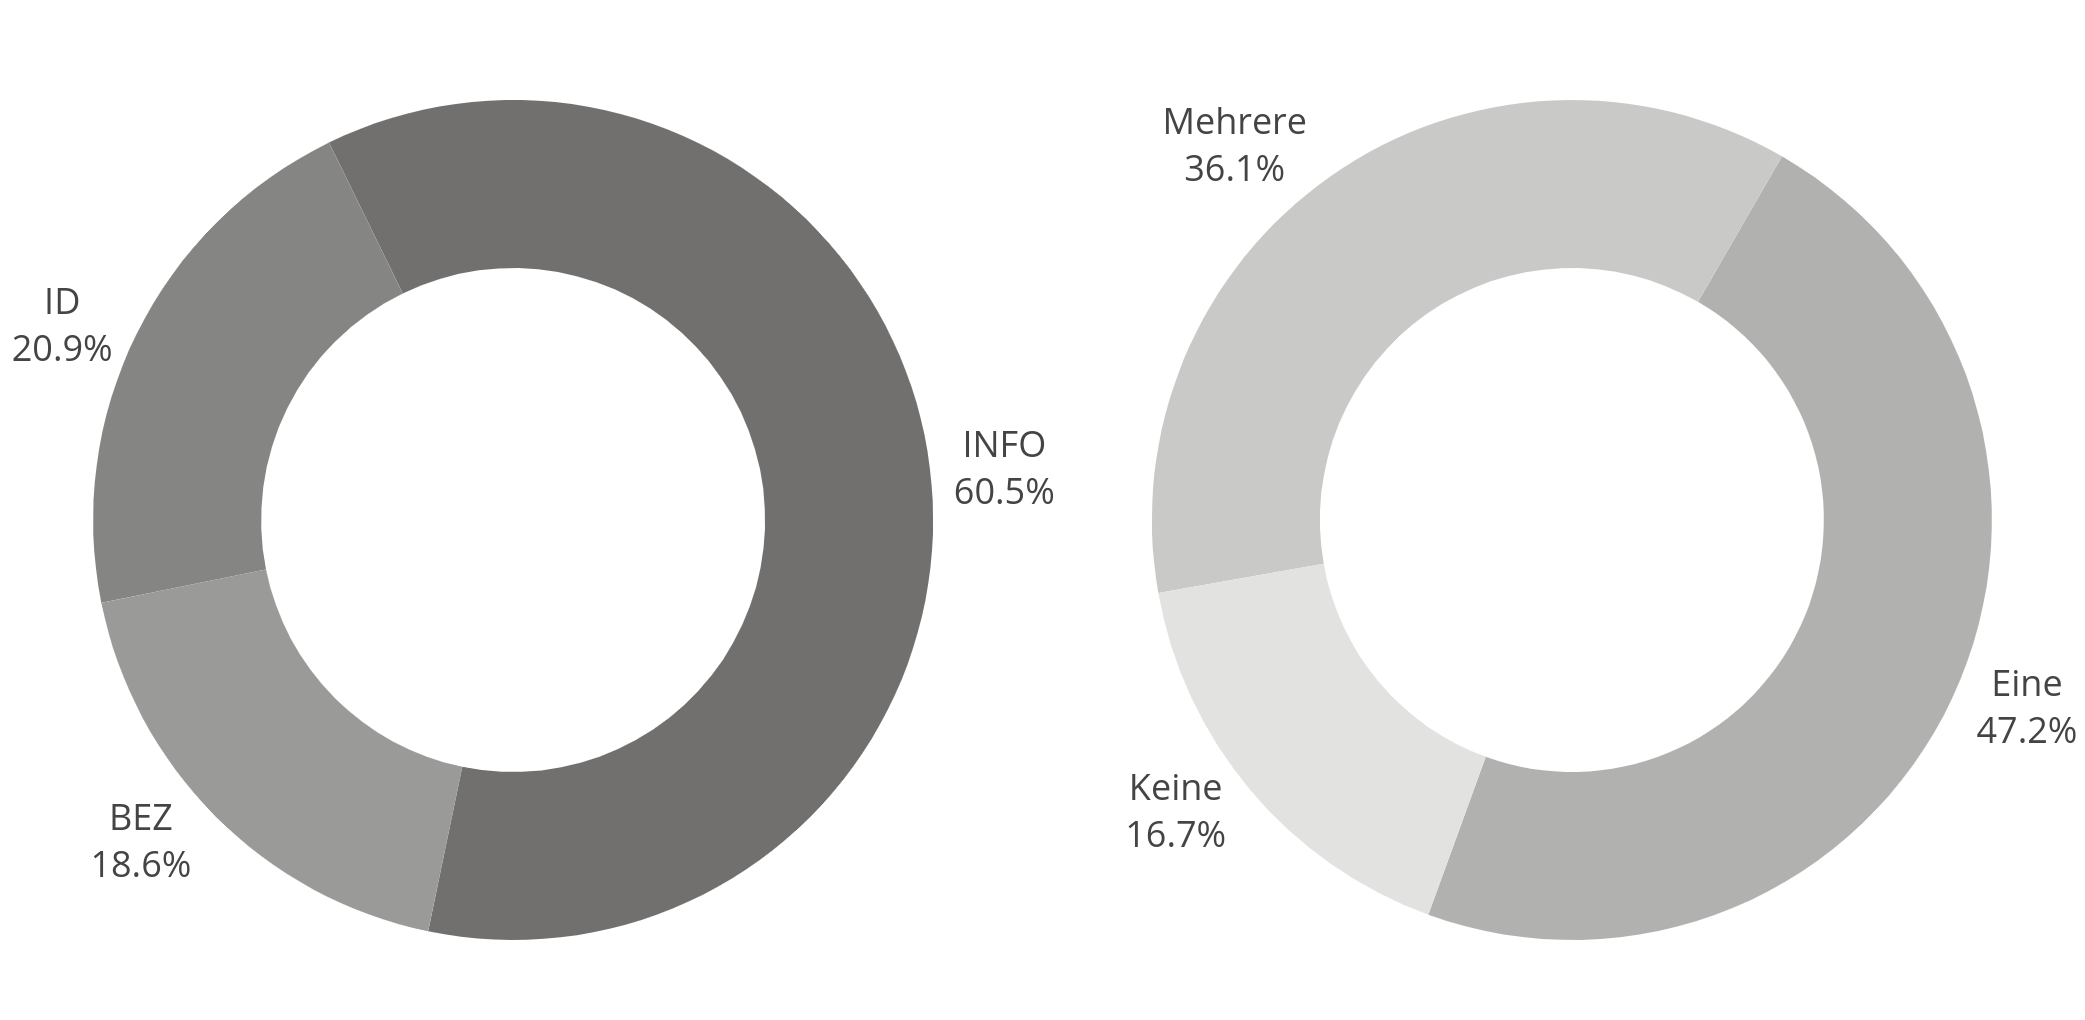
\includegraphics[width=.9\textwidth]{img/plots/kat/kat_fb.png}
    \caption{Prozentuale Verteilung der Facebook-Beiträge in die Management-Leistungen nach Jan-Hinrik Schmidt. Links die Kategorisierung nach Management-Leistungen, rechts die Angabe, wie häufig Zuteilungen zu Management-Leistungen gemacht werden konnten.}
    \label{fig:kategoriefb}
\end{figure}  

\subsubsection{Blog}

Tabelle \ref{tab:kategoriebl} zeigt die Einteilung der Blog-Beiträge der Universität Bielefeld im Juli 2018 in die in \ref{sec:jhsforschung} eingeführten Management-Leistungen. Wie (auch in Abbildung \ref{fig:kategoriebl}) zu sehen ist, sind alle Beiträge des Blogs mindestens der Kategorie Informationsmanagement zugeordnet. Ein Beitrag kann zusätzlich dem Beziehungsmanagement zugeordnet werden. Wie die Abbildung \ref{fig:kategoriebl} zeigt, handelt es sich dabei um einen Anteil von 2.17 \% an der Gesamtheit der Blog-Beiträge. 34.8 \% der Beiträge wurden neben dem Informationsmanagement auch dem Identitätsmanagement zugeordnet. Der rechte Teil der Abbildung \ref{fig:kategoriebl} zeigt außerdem die ausgeglichene Verteilung von Einfach- und Mehrfachzuordnungen in die Management-Leistungen.

\begin{table}[H]
    \caption{Blog Beiträge der Universität Bielefeld im Juli 2018 und ihre Zuordnung zu den Management-Leistungen nach Schmidt.}
\resizebox{\textwidth}{!}{%
\begin{tabular}{*{29}{c|}c}
 & \rotatebox{270}{BL\_02\_01 } & \rotatebox{270}{BL\_02\_02} & \rotatebox{270}{BL\_02\_03} & \rotatebox{270}{BL\_03\_01} & \rotatebox{270}{BL\_04\_01} & \rotatebox{270}{BL\_04\_02} & \rotatebox{270}{BL\_05\_01} & \rotatebox{270}{BL\_05\_02} & \rotatebox{270}{BL\_05\_03} & \rotatebox{270}{BL\_06\_01} & \rotatebox{270}{BL\_10\_01} & \rotatebox{270}{BL\_10\_02} & \rotatebox{270}{BL\_11\_01} & \rotatebox{270}{BL\_12\_01} & \rotatebox{270}{BL\_13\_01} & \rotatebox{270}{BL\_16\_01} & \rotatebox{270}{BL\_16\_02} & \rotatebox{270}{BL\_17\_01} & \rotatebox{270}{BL\_17\_02} & \rotatebox{270}{BL\_18\_01} & \rotatebox{270}{BL\_20\_01} & \rotatebox{270}{BL\_24\_01} & \rotatebox{270}{BL\_25\_01} & \rotatebox{270}{BL\_26\_01} & \rotatebox{270}{BL\_26\_02} & \rotatebox{270}{BL\_27\_01} & \rotatebox{270}{BL\_30\_01} & \rotatebox{270}{BL\_30\_02} & \rotatebox{270}{BL\_31\_01} \\
 \hline
ID &  & X & X & X & X &  &  & X & X & X &  &  & X &  &  & X &  &  & X &  &  & X & X & X &  & X & X &  & X \\
\hline
BEZ &  &  &  &  &  &  &  &  &  &  &  &  &  &  &  &  &  &  &  &  &  &  &  &  & X &  &  &  &  \\
\hline
INFO & X & X & X & X & X & X & X & X & X & X & X & X & X & X & X & X & X & X & X & X & X & X & X & X & X & X & X & X & X
\end{tabular}%
}
\label{tab:kategoriebl}
\end{table}

\begin{figure}[H]
    \centering
    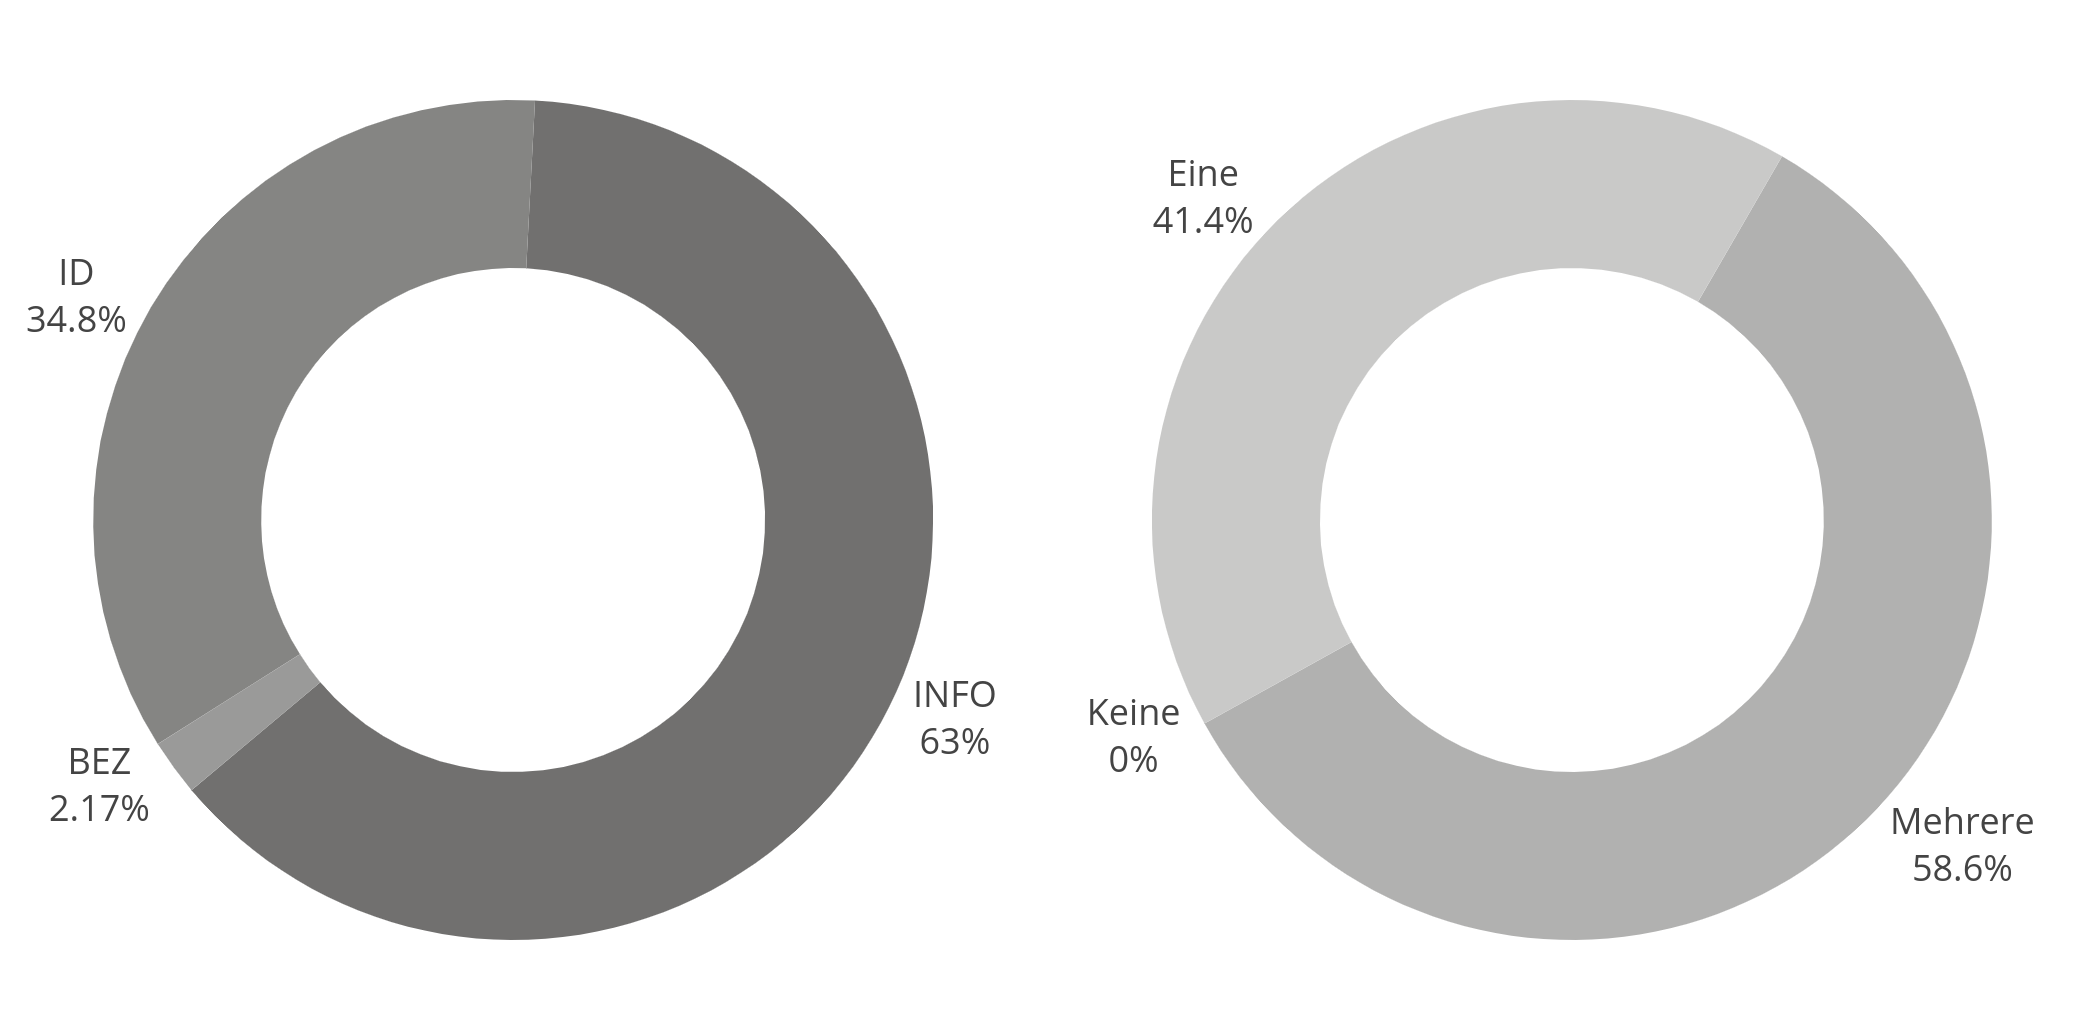
\includegraphics[width=.9\textwidth]{img/plots/kat/kat_bl.png}
    \caption{Prozentuale Verteilung der Blog-Beiträge in die Management-Leistungen nach Jan-Hinrik Schmidt. Links die Kategorisierung nach Management-Leistungen, rechts die Angabe, wie häufig Zuteilungen zu Management-Leistungen gemacht werden konnten.}
    \label{fig:kategoriebl}
\end{figure}  

\subsubsection{Twitter}

Wie in Tabelle \ref{tab:kategorietw} zu sehen ist, wurde Twitter im untersuchten Monat nicht zum Beziehungsmanagement verwendet. Sechs von sieben Beiträgen auf Twitter folgen dem Informationsmanagement, vier dem Identitätsmanagement. Ein Beitrag ist keiner der Kategorien zuzuordnen. Wie in den oberen Abschnitten über Facebook und den Universitäts-Blog auch, lassen sich in der hier aufgezeigten Abbildung \ref{fig:kategorietw} die Aufteilungen in die Management-Leistungen ablesen. 

\begin{table}[h]
    \caption{Blog Beiträge der Universität Bielefeld im Juli 2018 und ihre Zuordnung zu den Management-Leistungen nach Schmidt.}
\resizebox{\textwidth}{!}{%
\begin{tabular}{*{7}{c|}c}
 & TW\_03\_01 & TW\_10\_01 & TW\_11\_01 & TW\_13\_01 & TW\_25\_01 & TW\_27\_01 & TW\_30\_01 \\
 \hline
ID & X &  & X &  & X & X &  \\
\hline
BEZ &  &  &  &  &  &  &  \\
\hline
INFO & X & X & X & X & X & X & 
\end{tabular}%
}
\label{tab:kategorietw}
\end{table}

\begin{figure}[h]
    \centering
    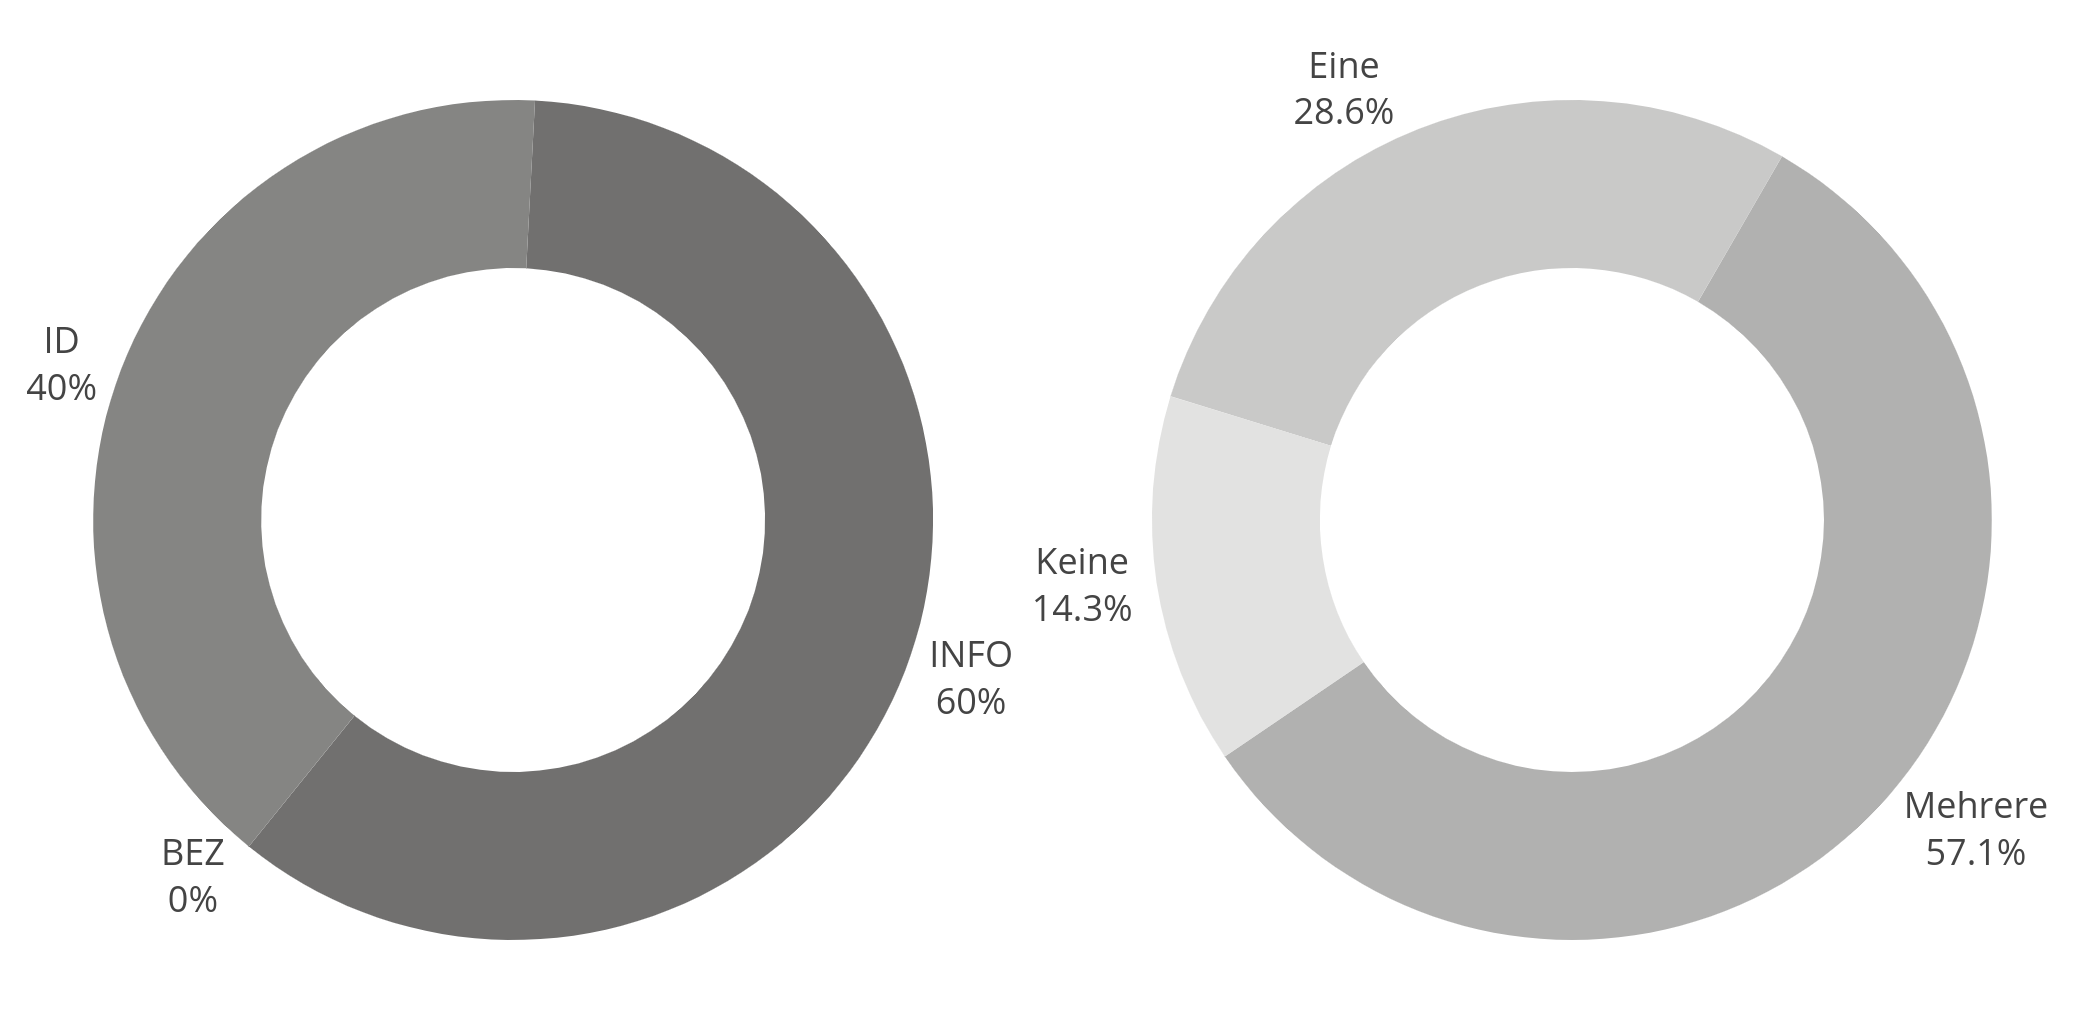
\includegraphics[width=.9\textwidth]{img/plots/kat/kat_tw.png}
    \caption{Prozentuale Verteilung der Twitter-Beiträge in die Management-Leistungen nach Jan-Hinrik Schmidt. Links die Kategorisierung nach Management-Leistungen, rechts die Angabe, wie häufig Zuteilungen zu Management-Leistungen gemacht werden konnten.}
    \label{fig:kategorietw}
\end{figure}  

\section{Ergebnisse}
\label{sec:Ergebnisse}

% Darstellung der Auswertung der Daten. Hier wird nicht interpretiert. Es werden nicht die Hypothesen beantwortet. - beschreibende Daten

Tabelle \ref{tab:socialmediapostsprozent} zeigt, dass mit 36 Beiträgen, Facebook \printpercent{36}{105} aller Beiträge ausmacht. Twitter ist mit sieben Beiträgen, und damit \printpercent{7}{105}, der im Juli 2018 am wenigsten genutzte Social Web Kanal der Universität. YouTube-Videos machen \printpercent{11}{105}, Instagram-Beiträge \printpercent{22}{105}, und Blog-Beiträge \printpercent{29}{105} der Social Web Beiträge aus.

\begin{table}[H]
    \centering
    \caption{Prozentuale Verteilung der Social Web Beiträge der Universität Bielefeld im Juli 2018.}
        \begin{tabular}{*{5}{l}}
        Facebook & Universitäts-Blog & Instagram & YouTube & Twitter \\
        \hline
        \printpercent{36}{105} & \printpercent{29}{105} & \printpercent{22}{105} & \printpercent{11}{105} & \printpercent{7}{105}
    \end{tabular}
    \label{tab:socialmediapostsprozent}
\end{table}

Im Gegensatz zu der relativ eindeutigen Follower-Verteilung (Abbildung \hyperref[fig:follower]{\ref{fig:follower} \& Tabelle \ref{tab:followerprozent}}), die einen starken Überhang an Facebook-Followern gegenüber allen anderen Plattformen zeigt, sind die Beiträge -- mit Ausnahme der Twitter-Beiträge -- eher gleichmäßig verteilt.

Von den 105 Beiträgen, die die Universität im Juli über alle Plattformen veröffentlicht hat, wurden in Abschnitt \ref{sec:jhseinteilung} die auf Text basierten 72 Beiträge der Plattformen Facebook, Twitter und Universitäts-Blog untersucht und kategorisiert. Von den 72 untersuchten Beiträgen konnten, wie in Abbildung \ref{fig:kategorietext} zu sehen, 43.1 \% der Beiträge eindeutig einer Kategorie zugeordnet werden. Bei etwa 47 \% der Beiträge ließen sich zwei oder sogar drei Kategorien zuteilen. Fast 10 \% aller Beiträge konnten jedoch keiner der drei Management-Leistungen uneingeschränkt zugewiesen werden.

\begin{figure}[H]
    \centering
    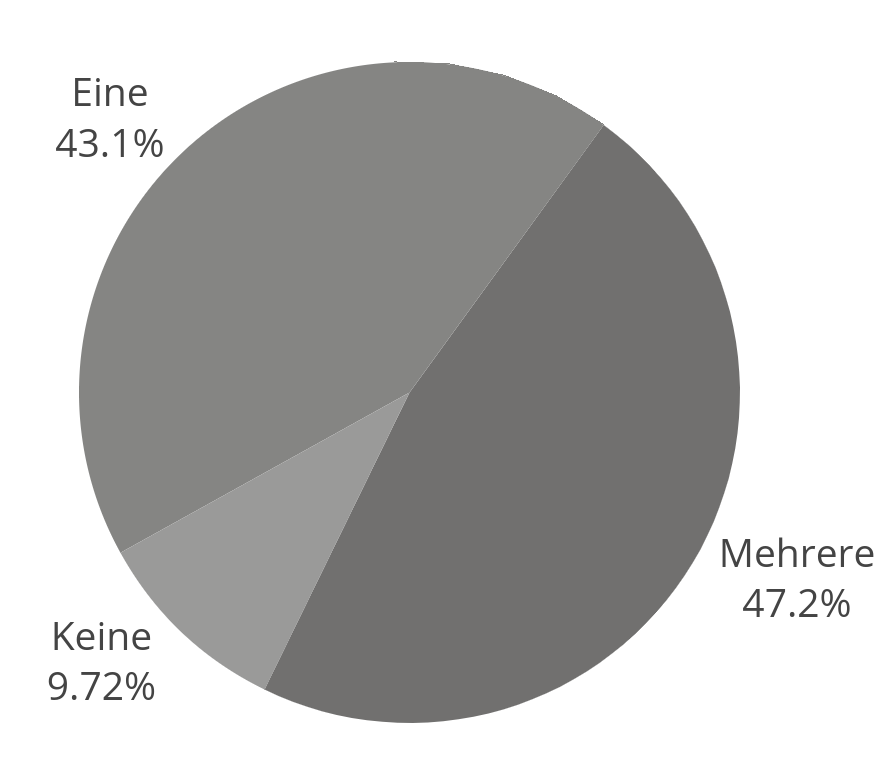
\includegraphics[width=.5\textwidth]{img/plots/kat/kat_text.png}
    \caption{Prozentuale Verteilung der Zuordnungshäufigkeit der auf Text basierten Social Web Beiträge in die Management-Leistungen. Der Datensatz umfasst 72 Beiträge.}
    \label{fig:kategorietext}
\end{figure}  

Abbildung \ref{fig:kategorietextprozent} zeigt, dass der Großteil der Beiträge im Kern Informationsbeiträge gewesen sind. Knapp 72 \% aller Facebook-, über 85 \% aller Twitter- und ohne Ausnahme alle Blog-Beiträge konnten mit dem Informationsmanagement kategorisiert werden. Der Anteil an Beziehungsmanagement ist bei Facebook mit 22.22 \% am höchsten. Nur 3.45 \% des Blog-Beiträge haben -- zum Beispiel durch den Aufruf zu Mitarbeiten, Veranstaltungen, und Ähnlichem -- Beziehungsmanagement betrieben. Bei den Twitter-Beiträgen im Juli konnte kein Beitrag dieser Kategorie zugeordnet werden. Dem Identitätsmanagement konnten von den Facebook-Beiträgen ein Viertel, und mit jeweils 55.17 \% und 57.14 \% knapp über die Hälfte der Blog- und Twitter-Beiträge zugeordnet werden.

\begin{figure}[h]
    \centering
    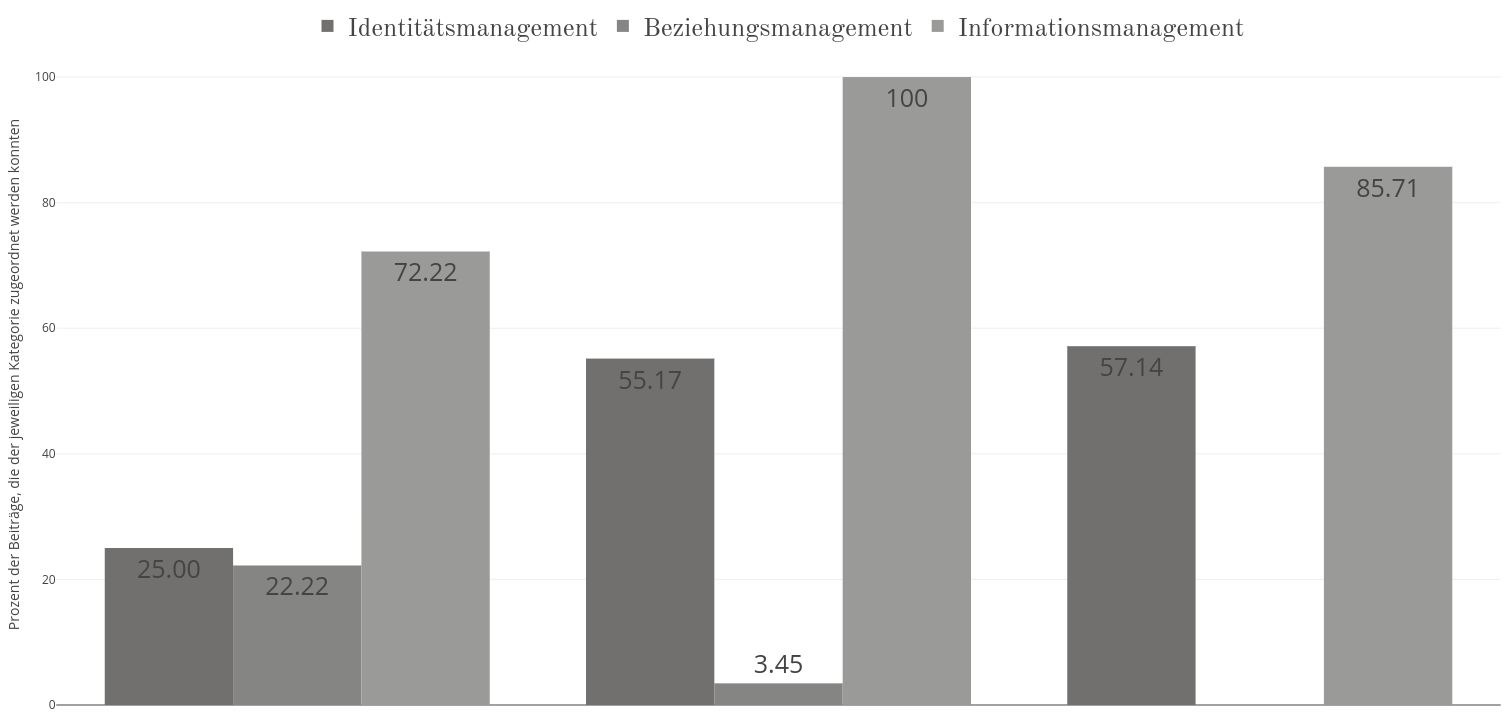
\includegraphics[width=\textwidth]{img/plots/kat/kat_text_prozent.png}
    \caption{Prozentuale Verteilung der Zuordnungshäufigkeit der auf Text basierten Social Web Beiträge in die Management-Leistungen. Der Datensatz umfasst 72 Beiträge. Der linke Teilgraph zeigt Facebook-Beiträge, der mittlere Blog-Beiträge und der rechte Twitter-Beiträge.}
    \label{fig:kategorietextprozent}
\end{figure} 

\section{Diskussion}
\label{sec:Diskussion}

% Zusammenfassung der Ergebnisse - Hypothesen bestätigt? Falsifiziert? (Bewertung) - Fragestellung geklärt? - Theoriebedeutung - Kurze Praxisbedeutung - Kritische Diskussion der Ergebnisse - Mängel / Verbesserungen der Studie

Mit der stetig wachsenden Nutzung von Social Web Plattformen, machen immer häufiger auch Firmen, Vereine und Institutionen Gebrauch vom Potenzial der einfachen Erreichbarkeit über das Internet; ob für die Wertsteigerung des Unternehmens oder im Personalmanagement (vgl. \cite{culnan2010large} \& \cite{barmann2016social}). Schaut man sich die größten Universitäten des Landes an, haben alle bis auf sehr wenige Ausnahmen mindestens dasselbe Social Web Repertoire, wie die Universität Bielefeld. Herausstechen tut die Universität Duisburg Essen, die zusätzlich dazu noch Snapchat, Google+, Flickr, XING, LinkedIn und sogar eine eigene Campus-App bereitstellt\footnote{Universität Duisburg-Essen -- \url{https://www.uni-due.de/}}. Das Angebot der verschiedenen Social Web Plattformen steigt -- wie man an der Universität Duisburg-Essen gut sieht -- immer weiter, weshalb sich gerade Institutionen, die sich nur eine durch das Personal eingeschränkte Bespeisung der Netzwerke leisten können, im Normalfall auf einige wenige Plattformen beschränken müssen. Die Universität Bielefeld hat auf den verschiedenen Social Web Plattformen insgesamt 34.140 Follower. Davon fallen knapp die Hälfte Facebook zu. Knapp 7.000 Nutzerinnen und Nutzer folgen der Universität Bielefeld auf Instagram, und etwas über 6.000 Follower kann der Universitäts-Twitter-Account verzeichnen. Den YouTube-Kanal der Universität abonnierten, Stand September 2018, nur 800 Personen. Diese 34.140 Follower werden von sechs Mitarbeiterinnen und Mitarbeitern der Universität unterhalten\footnote{\href{https://ekvv.uni-bielefeld.de/pers_publ/publ/EinrichtungDetail.jsp?orgId=7116054}{Abteilung \textit{Medien und News}, Referat für Kommunikation}}.

Die Analyse des vorliegenden Datensatzes der Social Web Beiträge der Universität Bielefeld aus dem Juli 2018 ergab, dass auch hier eine begründete Selektion stattfand. 72 der 105 untersuchten Beiträge wurden auf im Kern textbasierten Social Web Plattformen veröffentlicht. YouTube-Videos und Instagram-Bilder und -Videos stellen den etwas kleineren Teil der Beiträge dar und wurden für die inhaltliche Analyse mithilfe der Forschungen von Jan-Hinrik Schmidt (siehe \ref{sec:jhsforschung}) außer Acht gelassen.

Die 72 näher untersuchten Beiträge teilen sich in 50 \% Facebook-Beiträge, etwa 40 \% Blog-Beiträge und etwa 10 \% Twitter-Beiträge auf. Die 50 \% Facebook-Beiträge korrelieren hier sehr stark mit den oben genannten Follower-Zahlen. Bei allen anderen Plattformen ist eine solche Korrelation jedoch nicht erkennbar. Die etwas über 6.000 Twitter-Follower wurden in dem untersuchten Monat nur mit sieben Beiträgen beglückt, die sich teilweise auch mit Beiträgen der anderen Plattformen doppeln. Der YouTube-Kanal hat hingegen mit $1:72$ die höchste Rate von Beiträgen zu Abonnenten. Dies könnte damit erklärt werden, dass in der Gesamtheit die Zahl der YouTube-Videos weit unter der Zahl der Beiträge auf den anderen Social Web Plattformen liegt, und deshalb (noch) nicht viele Nutzerinnen und Nutzer von dem Kanal wissen oder regelmäßig die Videos schauen. Zudem ist die soziale Hürde einen YouTube-Kanal zu abonnieren, höher als die, eine Seite auf Facebook mit einem Like zu markieren. Zu den wenigen Abonnenten kommen dann in letzter Zeit  immer mehr Video-Beiträge, unter anderem durch Universitäts-Formate wie \textit{Campus TV}\footnote{Campus TV Universität Bielefeld -- \url{https://lul.uni-bielefeld.de/projekte/campustv}} oder das Seminar \textit{Vosicht Podcast!}, welches seit 2008\footnote{\href{https://uni-bielefeld.de/kvv_publ/publ/Lehrende_Veranstaltungen.jsp?personId=3772740}{Paul John -- Vorsicht Podcast!}} regelmäßig für verschiedenste Studiengänge angeboten wird.


Bei der Einordnung der Beiträge zu den Management-Leistungen der Social Web Anwendungen konnte gezeigt werden, dass 90 \% der Beiträge mindestens einer Leistung zugewiesen werden können. Bei knapp 10 \% der Beiträge war eine solche Zuordnung jedoch nicht möglich. Dies ist ein überaus signifikanter Teil der Beiträge. Die Fragestellungen aus Kapitel \ref{sec:hypothesen}, ob das Modell nach Jan-Hinrik Schmidt auf die Social Web Kommunikation der Universität Bielefeld anwendbar ist, und die Beiträge der Universität, wie die einer Einzelperson, in die drei Management-Leistungen Identitätsmanagement, Beziehungsmanagement und Informationsmanagement eindeutig zugeordnet werden können, müssen demnach beide verneint werden. 

Außerdem kann aus den Ergebnissen hergeleitet werden, dass die ebenfalls in Kapitel \ref{sec:hypothesen} erarbeitete Hypothese dieser Abschlussarbeit bestätigt werden kann. Das untersuchte Modell kann nach jetzigem Stand nicht ohne Überarbeitung auf die Social Web Kommunikation von Institutionen angewandt werden.

Dadurch, dass es sich um die Anwendung eines etablierten Modells auf einen Bereich handelt, der von dem Modell nicht intendiert gewesen ist, handelt es sich bei dem Ergebnis nicht um eine Kritik am Modell nach Jan-Hinrik Schmidt, sondern um die Feststellung, dass sich die Social Web Kommunikation einer Einzelperson von der einer Institution so weit unterscheidet, dass das Modell dort unüberarbeitet keine Anwendung finden kann.

Zuletzt möchte ich in diesem Kapitel -- trotz der Bestätigung der Arbeitshypothese -- kritisch auf den Aufbau der Arbeit schauen und Möglichkeiten aufzeigen, wie sich die Arbeit verbessern ließe. Zur Ermöglichung der Verarbeitung, wurde der untersuchte Datensatz auf einen Monat beschränkt. Auch wenn der Zeitraum in Abschnitt \ref{sec:Datenauswahl} begründet wurde, so bleibt dennoch die Frage nach der Repräsentativität des Datensatzes. Durch die händische Verarbeitung musste der Datensatz stark limitiert werden. Ein größerer Datensatz, beispielsweise über einen Zeitraum von einem ganzen Semester, würde repräsentativere Daten ergeben, und ermöglichen, eine bessere Einschätzung bekommen zu können, ob die Modell-Anwendbarkeit gegeben ist oder nicht. 
Im Rahmen dieser Arbeit wurden außerdem nur die textbasierten Social Web Plattformen untersucht; die visuell ausgerichteten Foto- und Video-Plattformen -- namentlich Instagram und YouTube -- wurden außer Acht gelassen. Dadurch gehen ebenfalls Daten verloren, die die Analyse und somit das Ergebnis der Arbeit beeinflussen hätten können. Eine händische Kategorisierung ist außerdem Fehlerbehaftet, da sie im Zweifelsfall nicht stark genug fixierten Regeln folgt. Die Aussagekraft der Einordnung in Kategorien in Abschnitt \ref{sec:jhseinteilung} ist demnach nicht fest reguliert und daher womöglich nicht aussagekräftig genug. 
Des Weiteren war die Datenauswahl auf Ursprungs-Beitrags-Daten beschränkt. Dies meint, dass Die Nutzerinnen- und Nutzer-Interaktionen, wie das Liken von Facebook-Beiträgen, das Retweeten von Twitter-Beiträgen und das Kommentieren im Allgemeinen nicht analysiert wurden und somit womöglich der Aspekt des Beziehungsmanagements nicht hinreichend bearbeitet wurde.

Die oben angesprochenen visuellen Plattformen aus der Analyse raus zu lassen, hatte im Rahmen dieser Arbeit den Umfang betreffende Praktikabilitätsgründe. Die Daten, die im Zuge dessen verloren gehen, ließen sich durch die Nutzung der von YouTube automatisch generierten Untertitel, oder, da diese recht ungenau sind (vgl. \cite{parton2016video}), durch vorherige Annotationsarbeiten wiederum verwendbar machen.  Dazu könnten beispielsweise Skripte der YouTube-Videos erstellt, oder auch die Instagram-Fotos mithilfe digitaler Bilderkennungssoftware verschlagwortet werden. Um den oben genannten Kritikpunkten an der Arbeit entgegen zu kommen, böte sich außerdem an, die Verarbeitung der Daten zu automatisieren. Damit ließe sich zum einen die Datenanalyse skalieren, bis hin zur Verarbeitung aller öffentlich zugänglichen Social Web Beiträge, und zum anderen auch die oben angesprochenen Annotationen der Bilder und Videos in die Datenverarbeitung mit einbeziehen.

Eine solche Automatisierung könnte dann über programmatisch festgelegte Kategorisierungsregeln oder mithilfe der Verarbeitung von großen Datenmengen mittels künstlicher Intelligenz und neuronaler Netzwerke erfolgen. Solch große Datenmengen würden dann die Repräsentativität der Analyseergebnisse nochmals verbessern können.